\documentclass[runningheads,a4paper]{llncs}

\usepackage{amssymb}
\usepackage{graphicx} % Used for inserting pdf as graphics
\usepackage{subcaption}
%\usepackage{subfig}
\usepackage{float} % Used fo0r 'H' float option in figures
\usepackage{hyperref} % Used for creating a hyperlink to reference parts
\usepackage{textcomp}
\usepackage{multicol}
\usepackage{tikz}
\usepackage{multirow}
\usepackage{url}
\usepackage{color}
\usepackage{mathtools}
\usepackage[ruled,vlined,linesnumbered]{algorithm2e}

\usetikzlibrary{positioning}
\usetikzlibrary{shapes.multipart}
\usetikzlibrary{shapes.misc} % used for rounded rectangle

\let\proof\relax 
\let\endproof\relax 
\usepackage{amsthm}

\urldef{\mailsa}\path|radelacruz@up.edu.ph|
%\DeclarePairedDelimiter\ceil{\lceil}{\rceil}
%\DeclarePairedDelimiter\floor{\lfloor}{\rfloor}
    
\newcommand{\keywords}[1]{\par\addvspace\baselineskip
\noindent\keywordname\enspace\ignorespaces#1}

\theoremstyle{definition}
\newtheorem{definition2}{Definition}

% NEW COMMANDS =====================================================================================

\newcommand{\ra}{\rightarrow}
\newcommand{\se}{\text{ }}
\newcommand{\mn}{\text{-}}

\begin{document}

\mainmatter

\title
{
Homogenization of Spiking Neural P Systems
}

\titlerunning
{
Homogenization of SNP Systems
}


\author
{
Ren Tristan A. de la Cruz$^1$
}

\authorrunning {de la Cruz et al}


\institute
{
$^1$Algorithms and Complexity Laboratory \\
Department of Computer Science, University of the Philippines - Diliman\\
Diliman 1101, Quezon City, Philippines    \\
\mailsa ,
}


\toctitle{Lecture Notes in Computer Science}
\tocauthor{Authors' Instructions}


\maketitle

% ================================================================================================= %

\begin{abstract}

(ABSTRACT)

\keywords{Membrane Computing, 
          Spiking Neural P Systems, 
          Homogeneous Neurons,
          Structural Plasticity}
\end{abstract}



% ================================================================================================= %
\section{Introduction}
% ================================================================================================= %


% ================================================================================================= %
\section{Spiking Neural P System and Some Variants} \label{sec-snps}
% ================================================================================================= %


% ================================================================================================= %
\section{Homogenization of Spiking Neural P Systems} \label{sec-homo}
% ================================================================================================= %


% ================================================================================================= %
\subsection{Representing Neurons as Labelled Transition Systems}
% ================================================================================================= %

We will use the \emph{labelled transition system} construct to represent the activities and behavior 
of neurons in SNP systems. Each neuron in a SNP system will have a corresponding labelled transition 
system.

\begin{definition2}   [Labelled Transition System]   \label{def-lts}
A \emph{labelled transition system (LTS)} is a tuple $(S, L, \ra)$ where $S$ is a \emph{set of 
states}, $L$ is a \emph{set of labels}, and $\ra \subseteq S \times L \times S$ is a 
\emph{transition relation}.
\end{definition2}

We will call an LTS that represents an SNP system neuron as a \emph{neuron LTS}. Neuron LTSs use a 
particular set of states and a particular set of labels that are relevant to SNP systems.

%===================================================================================================

\emph{States} of neuron LTSs are a sets of natural numbers that represents sets of spike counts. 
For example, the state $\{4,5\}$ represents spike counts $4$ and $5$, the state $\{0,2,4,8,...\}$ 
represents even spike counts, and the state $\{15,20,25,30,...\}$ represents spike counts that 
are multiples of $5$ greater than or equal to $15$. Since a state $s$ is a set of natural numbers,
the set of states $S$ of some neuron LTS $(S,L,\ra)$ is a set of subsets of natural numbers. i.e.
For a neuron LTS $(S,L\ra)$, $S \subseteq \mathcal{P}(\mathbb{N})$ where $\mathcal{P}(\mathbb{N})$ 
is the power set of $\mathbb{N}$.

%===================================================================================================

\emph{Labels} of neuron LTSs represent receptions of spikes or rule applications. Labels will have
the form $(\alpha,\beta)$ where $\alpha$ is an integer that represents the number of spikes 
consumed if $\alpha < 0$ or the number of spikes received if $\alpha > 0$ while $\beta$ presents 
some action, spiking or forgetting, during rule application. For example, let labels with $\beta=0$
represent applications of forgetting rules while labels with $\beta=1$ represent applications of 
spiking rules, the label $(-3,0)$ represents the application of a forgetting rule that consumes $3$ 
spikes while the label $(-2,1)$ represents the application of a spiking rule that consumes $2$ 
spikes. Labels that represent receptions of spikes will have $\alpha > 0$ and $\beta=0$. For
example, the label $(4,0)$ represents the reception of $4$ spikes while the label $(1,0)$ represents
the reception of $1$ spike. 

For any label $(\alpha,\beta)$, $\alpha \in \mathbb{Z}$ while $\beta$ is an element of some 
\emph{set of actions} $\mathcal{A}$ that is relevant to SNP systems. In the previous examples, we
use $\mathcal{A}=\{0,1\}$ where $0$ represents a forgetting action and $1$ represents a spiking 
action. The assumption when using $\mathcal{A}=\{0,1\}$ as the set of actions is that we are only 
dealing with SNP systems that do not use delays (all spiking rules have delays set to $0$). For 
SNP systems in general, $\mathcal{A} \subseteq \mathbb{N}$ can be used as the set of actions. For a 
$\beta \in \mathcal{A}$, if $\beta=0$ then $\beta$ represents a forgetting action and if $\beta=d>0$
then $\beta$ represents a spiking action with $d\mn 1$ delay. For SNP systems with extended rules, 
$\mathcal{A} \subseteq \mathbb{N} \times \mathbb{N}$ can be used as the set of actions. $\beta=(p,d) 
\in \mathcal{A}$ represents an action of producing $p$ spikes after a $d$ delay. For example, 
$\beta=(3,2)$ represents the action of producing $3$ spikes after $2$ steps, $\beta=(5,0)$ 
represents the action of producing $5$ spikes immediately, and $\beta=(0,0)$ represents the 
forgetting action. For SNP systems with extended rules, we can have labels like $(-6,(5,0))$ that
represents consumption of $6$ spikes and immediate production of $5$ spikes, $(-5,(3,2))$ that
represents consumption of $5$ spikes and production of $3$ spikes after $2$ steps, and $(-7,(0,0))$ 
that represents consumption of $7$ spikes (forgetting action). In general, the set of labels
that will be used by neuron LTSs is  $L \subseteq \mathbb{Z} \times \mathcal{A}$ where $\mathcal{A}$
is a set of actions relevant to the SNP system variant.

%===================================================================================================

The \emph{transition relations} of neuron LTSs will contain \emph{transitions} of the form $(s, 
(\alpha,\beta), s')$ where $s$ and $s'$ are states and $(\alpha, \beta)$ is a label. The transition 
relation describes how the number of spikes in a neuron changes due to incoming spikes (events) or
due to rule applications (actions). If a neuron has $n$ spikes and $n \in s$, then we say that the
neuron \emph{is in state} $s$. The transition $(s,(\alpha,\beta),s')$ means that if the neuron is in
state $s$ and the event/action $(\alpha,\beta)$ occurred, then the neuron will transition to having 
$n+\alpha$ spikes which is state $s'$ (the neuron \emph{transitions to state} $s'$). For example,
the transition $(\{2,4,6,8,...\},(-1,1), \{1,3,5,7,...\})$ means that if the neuron has $n$ spikes 
which is even (the neuron is in the `even spike count' state) and the action $(-1,1)$ occurred (a 
spiking rule that consumes $1$ spike is applied), then the neuron will transition to having $n\mn 1$ 
spikes (the neuron transitions to the `odd spike count' state). The transition $(s,(\alpha,\beta),
s')$ can simply be written as $(s,(\alpha,\beta))$ because the next state $s'$ can be derived from 
the current state $s$ and the $\alpha$ component of the label $(\alpha,\beta)$. The next state is 
defined as $s'=\{n+\alpha\se|\se n \in s\}$.

%===================================================================================================

For a transition $(s,(\alpha,\beta))$ that represents an SNP system rule, state $s$ represents the
set of spike counts where the rule is applicable, $\alpha<0$ represents the number of spikes the
rule consumes, and $\beta$ represents the action performed by the rule (spiking or forgetting). 
Figure \ref{fig-lts-1} shows two examples of neurons and their LTSs. Figure \ref{fig-lts-1a} shows
neuron $w$ with two incoming synapses, one from neuron $x$ and another from neuron $y$, and it 
contains the rules $a/a \ra \lambda$ and $a^2/a^2\ra a$. Rule $a/a\ra \lambda$ is represented by the 
transition $(\{1\},(-1,0))$. The state $\{1\}$ means the rule can only be applied when the neuron 
has $1$ spike. The label $(-1,0)$ means the rule consumes $1$ spike ($\alpha=-1$) and is a 
forgetting rule ($\beta = 0$). Rule $a^2/a^2\ra a$ is represented by the transition $(\{2\},
(-2,1))$. The state $\{2\}$ means the rule can only be applied when the neuron has $2$ spikes while
the label $(-2,1)$ means the rule is a spiking rule that consumes $2$ spikes. In Figure 
\ref{fig-lts-1a} and the rest of the figures with LTS, a state is drawn as set of numbers inside a
rectangle and a label is drawn as an arrow. The transition $(\{0\},(+1,0))$ represents the reception 
of one spike while the neuron has $0$ spikes while the transition $(\{0\},(+2,0))$ represents the
reception of $2$ spikes while the neuron has $0$ spikes.

Figure \ref{fig-lts-1b} shows another example of a neuron and its LTS. Figure \ref{fig-lts-1b} shows
neuron $w$ with two incoming synapses, one from neuron $x$ and another from neuron $y$, and it 
contains the rules $a(a^2)^+/a^3 \ra a$ and $a/a\ra \lambda$. Rule $a(a^2)^+/a^3 \ra a$ is 
represented by the transition $(\{3,5,7,9,...\},(-3,1))$ which means it is applicable when the 
neuron has an odd number of spikes equal that is at least $3$, it consumes $3$ spikes ($\alpha=-3$),
and it is a spiking rule ($\beta=1$). Rule $a/a \ra \lambda$ is represented by the transition 
$(\{1\},(-1,0))$ which means it is only applicable when the neuron has $1$ spikes and it is a
forgetting rule ($\beta=0$) that consumes $1$ spike ($\alpha=-1$). The transition $(\{0,2,4,6,...\},
(+2,0))$ means that if then neuron has even number of spikes (in the even state) and it receives
$2$ spikes ($\alpha=+2$) the neuron will simply stay in the even state. The transition $(\{0,2,4,6,
...\},(+1,0))$ means that if the neuron is in the even state and it receives $1$ spike then the
neuron will transition to the odd state (neurons will now have odd number of spikes). 

\begin{figure}[h]
   \centering
   \begin{subfigure}{\textwidth}
      \centering
      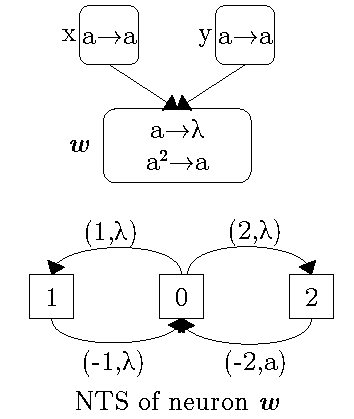
\includegraphics[scale=0.65]{fig-lts-1a.pdf}
      \caption{}
      \label{fig-lts-1a}
   \end{subfigure}
   \begin{subfigure}{\textwidth}
      \centering
      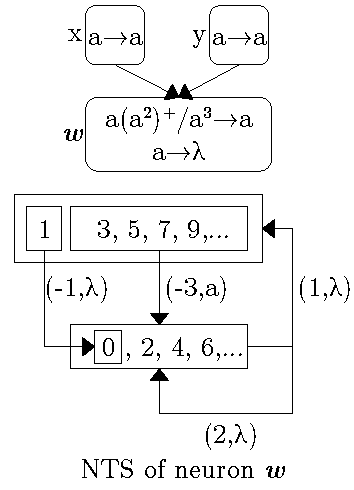
\includegraphics[scale=0.65]{fig-lts-1b.pdf}
      \caption{}
      \label{fig-lts-1b}
   \end{subfigure}
   \caption{Examples of Neurons and their LTSs}
   \label{fig-lts-1}
\end{figure}

%===================================================================================================

To construct the LTS of some neuron $w$, you need to know its rule set and the behavior of the
subsystem of neurons connected to neuron $w$ (neurons that have synapses going to neuron $w$). From 
the rule set, you get the transitions that represent the rules. The other transitions that represent 
receptions of spikes are derived from the behavior of subsystem of neurons connected to neuron $w$.
This means that neurons with the same rule set may have different LTSs. Figure \ref{fig-lts-2} shows 
two different LTSs for neuron $w$. In Figures \ref{fig-lts-2a} and \ref{fig-lts-2b}, neuron $w$ has 
the single rule $a^3/a^3 \ra a:0$ but the subsystem connected to neuron $w$ in Figure 
\ref{fig-lts-2a} is different from the subsystem connected to neuron $w$ in Figure \ref{fig-lts-2b}.
In Figure \ref{fig-lts-2a}, neurons $x$, $y$, and $z$ give one spike each to neuron $w$ one spike at
a time. The transition $(\{0\},(+1,0))$ represents neuron $x$ sending one spike to neuron $w$ when
neuron $w$ has $0$ spike. The transition $(\{1\},(+1,0))$ represents neuron $y$ sending a spike to
neuron $w$ when neuron $w$ has one spike. And, the transition $(\{2\},(+1,0))$ represents neuron
$z$ sending a spike to neuron $w$ when neuron $w$ has two spikes. Those $3$ transitions along with
the transition $(\{3\},(-3,1))$ for the rule are all the transitions for neuron $w$'s LTS.

In Figure \ref{fig-lts-2b}, starting with neuron $w$ having $0$ spikes, there are 4 scenarios that 
lead to neuron $w$ having $3$ spikes and these scenarios are: (scenario 1) neurons $x,y,z$ send one 
spike each to neuron $w$ at the same time [transition sequence: $(\{0\},(+3,0))$], (scenario 2) 
neuron $x$ sends a spike, then neurons $y$ and $z$ send a spike each at the same time [transition 
sequence: $(\{0\},(+1,0)),(\{1\},(+2,0))$], (scenario 3) neurons $x$ and $y$ send one spike each to 
neuron $w$ at the same time, then neuron $z$ sends a spike [transition sequence: ($\{0\},(+2,0)),
(\{2\},(+1,0))$)], and (scenario 4) neuron $x$ sends one spike follow by neuron $y$ sending another
spike then neuron $z$ sends the third spike [transition sequence: $(\{0\},(+1,0)),$ $(\{1\},(+1,0)),
(\{2\},(+1,0))$]. The two subsystems in Figure \ref{fig-lts-2} produce different sequences of events
which means different sets of transitions and therefore different LTSs for neuron $w$.

\begin{figure}[h]
   \centering
   \begin{subfigure}{\textwidth}
      \centering
      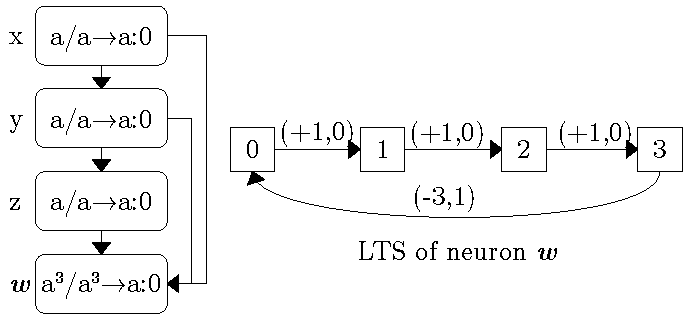
\includegraphics[scale=0.65]{fig-lts-2a.pdf}
      \caption{Neuron $w$ in a subsystem and neuron $w$'s LTS}
      \label{fig-lts-2a}
   \end{subfigure}
   \begin{subfigure}{\textwidth}
      \centering
      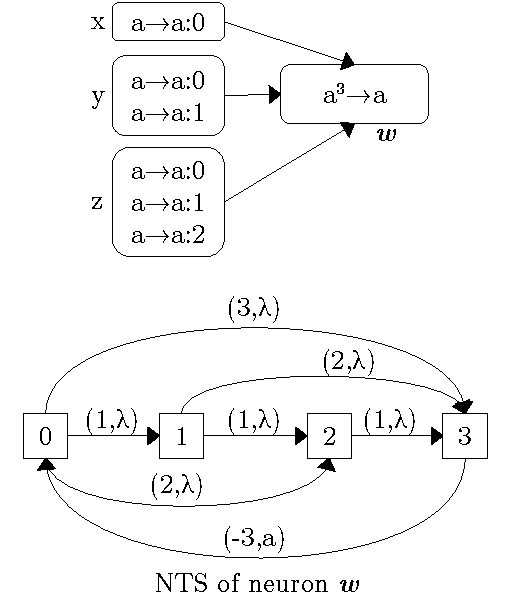
\includegraphics[scale=0.65]{fig-lts-2b.pdf}
      \caption{Neuron $w$ in a different subsystem with a different LTS}
      \label{fig-lts-2b}
   \end{subfigure}
   \caption{Neurons with same rule set but different LTSs}
   \label{fig-lts-2}
\end{figure}

%===================================================================================================
\subsection{Operations on Labelled Transition Systems}
%===================================================================================================

We will define two operations on labelled transition systems, \emph{LTS translation} and \emph{LTS
scaling}. The idea behind these operations is that they take an LTS and a parameter $\delta$ and 
produce a new LTS that behaves exactly like the original LTS. When you are combining two different
rule sets from two different neurons in order to have common rule set, simply getting the union of
the two rule sets can cause conflicts. For example, let $\{a \ra a, a^2/a\ra a\}$ be the rule set 
of neuron $x$ and $\{a\ra\lambda,a^2/a\ra a\}$ be the rule set of neuron $y$. If we simply combine
the rule sets to have the common rule set $\{a\ra\lambda,a\ra a, a^2/a\ra a\}$ for both neurons
$x$ and $y$, there will be an unwanted behavior. If neuron $x$ has $1$ spike it
should use the rule $a\ra a$ and if neuron $y$ has $1$ spike it should use the rule $a\ra \lambda$.
If neurons $x$ and $y$ use the common rule set, when they have $1$ spike both of them will have
a non-deterministic choice, use rule $a\ra \lambda$ or use rule $a\ra a$. This non-determinism is 
an unwanted behavior that is the result of rule $a\ra\lambda$ `conflicting' with rule $a\ra a$. The 
common rule set changes the behavior of both neuron $x$ and neuron $y$. LTS translation and LTS 
scaling will be used to avoid such conflicts and changes in the neurons' behavior when combining
different rule sets. 

\begin{definition2}[State Translation] 
\emph{State translation} is an operation on a state. It takes a state $s$ and a natural number 
$\delta$ and produces the state $s'$ defined as $s' = \{n + \delta\se|\se n \in s\}$. We
denote state translation with the $+$ symbol. i.e. $s+\delta = \{n + \delta\se|\se n \in s\}$.
We say that $s'$ is \emph{$s$ translated by $\delta$}.
\end{definition2}

For example, if $s_1=\{3,5,7\}$ and $\delta_1 = 3$, then $s_1+\delta_1 = s_1+3 = \{6,8,10\}$. If
$s_2 = \{3,6,9, 12,...\}= \{3i\}_{i\geq 1}$ and $\delta_2 = 2$, then $s_2+\delta_2 = s_2+2 = 
\{5,8,11,14,...\}$ $=\{3i+2\}_{i\geq 1}$. If $s_3 = \{1,3,5,7,...\} =\{2i-1\}_{i\geq 1}$ and 
$\delta_3=1$, then $s_3+\delta_3 = s_3 + 1 = \{2,4,6,8,..\}=\{2i\}_{i\geq 1}$.

\begin{definition2}[Transition Translation]
\emph{Transition translation} is an operation on a transition. It takes a transition $t = (s,
(\alpha,\beta))$ and a natural number $\delta$ and produces the transition $t'=(s',(\alpha,i
\beta))$ where $s'=s+\delta$ (state $s$ is translated by $\delta$). We also will use the same symbol 
$+$ for transition translation. i.e. $t' = t +\delta$. We say that $t'$ is \emph{$t$ translated by
$\delta$}.
\end{definition2}

A translation of the transition $(s,(\alpha,\beta))$ simply involves the translation of the state
$s$ component. The label component $(\alpha,\beta)$ is not modified. Since some transitions 
represent rules, the change due to transition translation has a corresponding change to the rule
that transition represents. If transition is translated by $\delta$, the regular expression $E$
of the rule is also translated by $\delta$. i.e. $a^{\delta}E$ is $E$ translated by $\delta$. For
example, if $E=a(a^2)^*$ then $E$ translated by $\delta$ is $a^{\delta}a(a^2)^*=a^{\delta+1}
(a^2)^*$. Let $r$ be the rule $E/a^c \ra \beta$ (where $\beta$ is some action e.g. spiking,
forgetting, spiking with delay, etc). We say some rule $r'$ is rule $r$ \emph{translated by 
$\delta$} if $r'$ is the rule $a^{\delta} E/a^c \ra \beta$. We will call this operation 
\emph{rule translation} which is the exact analogue of transition translation.

\begin{definition2}[LTS Translation]
\emph{LTS translation} is an operation on an entire transition system. It takes a labelled 
transition system $lts=(S,L,\ra)$ and a natural number $\delta$ and produces the labelled transition 
system $lts'=(S',L,\ra')$ where $S'=\{s+\delta\se|\se s \in S\}$ and $\ra' = \{t+\delta\se|\se t \in 
\ra\}$. We also use the same symbol $+$ for LTS translation. i.e. $lts'=lts+\delta$. We say that 
$lts'$ is \emph{$lts$ translated by $\delta$}.
\end{definition2}

The translation of $lts=(S,L,\ra)$ simply involves the translation of all transitions in the 
relation $\ra$ by the same amount $\delta$. This implies a change of the set of states $S$. The set 
of labels $L$ is unchanged.  

When you translate a neuron LTS, the translated LTS represents the same neuron behavior as the 
original LTS but the translated LTS is for a different neuron. The translated LTS is for the 
\emph{translated neuron}. Let some neuron $w$ have an initial number of spike $n$. We say some 
neuron $w'$ is neuron $w$ \emph{translated by} $\delta$ if neuron $w'$ has $n+\delta$ initial number 
of spikes and contains $\delta$-translated rules of neuron $w$. We will call this operation 
\emph{neuron translation} which is the exact analogue of LTS translation. Figure \ref{fig-lts-3} 
shows neuron $w'$ which is a $\delta$-translated neuron $w$ from Figure \ref{fig-lts-1a}. It also
shows the LTS of neuron $w'$ which is a $\delta$-translated LTS of neuron $w$ from Figure
\ref{fig-lts-1a}. Neurons $w$ and $w'$ have the same behavior because for any sequence of events
(sequence of receptions of spikes) they will have the same sequence of actions (sequence of applied 
rules).

%===================================================================================================

\begin{figure}[h]
   \centering
   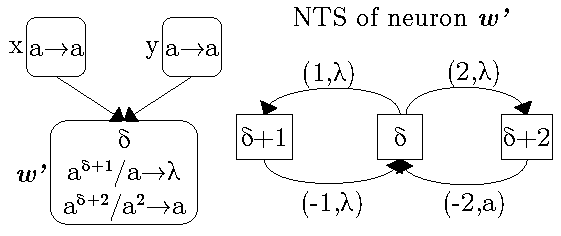
\includegraphics[scale=0.70]{fig-lts-3.pdf}
   \caption{Neuron $w'$ and its LTS}
   \label{fig-lts-3}
\end{figure}

\begin{lemma}
A neuron and a translated version of the neuron have the same behavior.
\end{lemma}

\begin{proof}
Let neuron $w'$ with LTS $lts'$ be a $\delta$-translated version of some neuron $w$ with LTS $lts$. 
If neuron $w$ has an initial $n_0$ spikes, then neuron $w'$ has an initial $n_0+\delta$ spikes. Let 
$T_0$ be the set of transition in $lts$ such that $(s,(\alpha,\beta))\in T_0$ if and only if 
$n_0\in s$. Let $T'_0$ be the corresponding set for $lts'$. i.e. $T_0'=\{(s',(\alpha',\beta'))\se|\se
n_0+\delta \in s'\}$. If $(s,(\alpha,\beta))\in T_0$, then $(s+\delta,(\alpha,\beta)) \in T'_0$ since
$n_0\in s$ and $n\in s$ implies $n_0+\delta \in s+\delta$. If  $(s+\delta,(\alpha,\beta)) \in T'_0$,
then $(s,(\alpha,\beta))\in T_0$ since $n_0+\delta \in s+\delta$ and $n_0+\delta \in s+\delta$ implies
$n_0\in s$ (by reversing the $\delta$-translation of state $s+\delta$). This means that the 
transitions in $T'_0$ are all $\delta$-translated transitions of $T_0$. Since transition translation
does not change the label $(\alpha,\beta)$, the transitions in $T_0$ has the same set of labels as
the transitions in $T'_0$. This means that neuron $w$ at $n_0$ spike count and neuron $w'$ at $n_0+
\delta$ have the same set of actions they can perform. The same argument can be used for when neuron
$w$ has spike count $n$ (which is not necessarily the initial spike count) while neuron $w'$ has
spike count $n+\delta$.
\end{proof}

%===================================================================================================

\begin{definition2}[State Scaling]
\emph{State scaling} is an operation on a state. It takes a state $s$ and a natural number
$\delta$ and produces the state $s'$ defined as $s' = \{\delta \cdot n\se|\se n\in s\}$. We
denote state scaling with the $\cdot$ symbol. i.e. $s'=\delta \cdot s$. We say that $s'$ is 
\emph{$s$ scaled by $\delta$}.
\end{definition2}

For example, if $s_1=\{1,2,3\}$ and $\delta_1=5$, then $\delta_1\cdot s_1 = 5\cdot s_1=\{5,10,15\}$.
If $s_2=\{2,4,6,8,...\}=\{2i\}_{i\geq 1}$ and $\delta_2=2$, then $\delta_2\cdot s_2=2\cdot s_2 =
\{4,8,12,16,...\}=\{4i\}_{i\geq 1}$. If $s_3=\{4,7,10,13,...\}=\{3i+1\}_{i\geq 1}$ and $\delta_3=2$,
then $\delta_3\cdot s_3 = 2\cdot s_3 = \{8,14,20,26,...\}=\{6i+2\}_{i\geq1}$.

\begin{definition2}[Transition Scaling]
\emph{Transition scaling} is an operation on a transition. It takes a transition $t=(s,(
\alpha,\beta))$ and a natural number $\delta$ and produces the transition $t'=(s',(\alpha',
\beta))$ where $s' = \delta \cdot s$ and $\alpha' = \delta \cdot \alpha$. We also use the $\cdot$
symbol for transition scaling. i.e. $t'=\delta\cdot t$. We say that $t'$ is \emph{$t$ scaled by 
$\delta$}.
\end{definition2}

Transition scaling scales both the state component $s$ and the $\alpha$ component (number of spikes
consumed or received) of the label $(\alpha,\beta)$ by the same factor $\delta$. Since some 
transitions represent rules, similar to transition translation there is a rule analouge for 
transition scaling which we will call \emph{rule scaling}. If $r$ is the rule $E/a^c \ra \beta$,
$r'$ is rule $r$ \emph{scaled by $\delta$}, written as $r'=\delta \cdot r$, if it is the rule
$E'/a^{\delta \cdot c} \ra \beta$ where $E'$ is the modified expression $E$ where all instances of 
expression $a$ is replace by expression $a^\delta$. For example, if $r$ is the rule $a(a^3)^*/a^2 \ra 
a$ with the corresponding transition $(\{3i+1\}_{i\geq 0},(-2,1))$ then
$r'=\delta \cdot r$ is the rule $(a^{\delta})((a^{\delta})^3)^*/a^{2\delta}\ra a$, or simply
$a^{\delta}(a^{3\delta})^*/a^{2\delta}\ra a$, with the corresponding transition $(
\{3i\delta+\delta\}_{i\geq 0},(-2\delta,1))$.

\begin{definition2}[LTS Scaling]
\emph{LTS scaling} is an operation on an entire transition system. It takes a labelled transition 
system $lts=(S,L,\ra)$ and a natural number $\delta$ and produces the labelled transition
system $lts'=(S',L',\ra')$ where $S' = \{\delta \cdot s\se|\se s\in S\}$, $L'=\{(\delta\cdot\alpha,
\beta\se)|\se (\alpha,\beta)\in L\}$, and $\ra' = \{\delta\cdot t\se|\se t \in \ra\}$. We also 
use the $\cdot$ symbol for LTS scaling. i.e. $lts'=\delta\cdot lts$. We say that $lts'$ is 
\emph{$lts$ scaled by $\delta$}.
\end{definition2}

%===================================================================================================

\begin{figure}[h]
   \centering
   \caption{Neurons with Same Rule Set but Different LTSs}
   \begin{subfigure}{\textwidth}
      \centering
      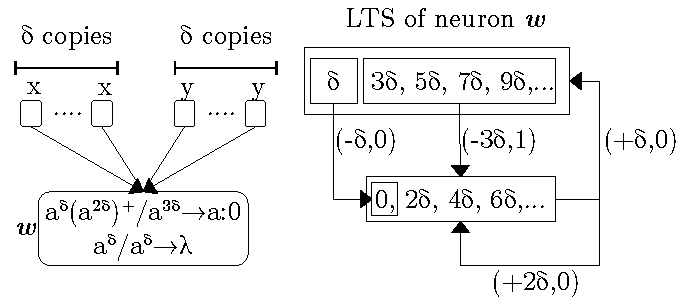
\includegraphics[scale=0.65]{fig-lts-4a.pdf}
      \caption{Neuron $w$ in a Subsystem and Neuron $w$'s LTS}
      \label{fig-lts-4a}
   \end{subfigure}
   \begin{subfigure}{\textwidth}
      \centering
      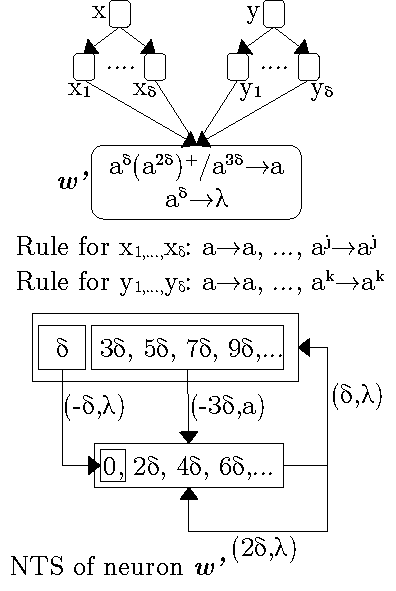
\includegraphics[scale=0.65]{fig-lts-4b.pdf}
      \caption{Neuron $w$ in a Different Subsystem with a Different LTS}
      \label{fig-lts-4b}
   \end{subfigure}
   \label{fig-lts-4}
\end{figure}

%===================================================================================================
\subsection{Procedures for Homogenizing Neurons' Rule Sets}
%===================================================================================================

\begin{definition2}[Rule Set]
A rule set $R$ is a set of rules $\{r_1,...,r_i,...,r_n\}$ where each rule $r_i$ has the form 
$(s_i,a_i)$. For rule $r_i=(s_i,a_i)$, $s_i$ is called the state while $a_i$ is called action.
The \emph{scope} of a rule set $R=\{(s_1,a_1),...,(s_n,a_n)\}$, denoted by $scope(R)$, is the state 
$s = s_1 \cup s_2 \cup \cdots \cup s_n$.
\end{definition2}

ELABORATE AND GIVE EXAMPLES(3)

\begin{definition2}[Scope Partitioning]
A partitioning of the scope of a rule set refers to the process of dividing the scope of the rule 
set into non-overlapping subsets. Let $R=\{(s_1,a_1),...,(s_n,a_n)\}$ be a rule with scope 
$s=scope(R)$. A partitioning of $s$, denoted by $part(s)$, is any set $\{\overline{s}_1,...,
\overline{s}_k\}$ such that:

\begin{itemize}
\item $\overline{s} \subseteq s$, 
      for each $\overline{s} \in part(s)$
\item $\overline{s}_x \cap \overline{s}_y = \varnothing$,
      for every $\overline{s}_x, \overline{s}_y \in part(s)$
\item $s = \bigcup\limits_{\overline{s}\in part(s)} \overline{s}$ ,
      $part(s) = \{\overline{s}_1,...,\overline{s}_k\}$
\end{itemize}

Any element of $\overline{s}$ of $part(s)$ is called a partition of $s$.

\end{definition2}

ELABORATE AND GIVE EXAMPLES(3)

\begin{definition2}[Actions]
Given a rule set $R=\{(s_1,a_1),...,(s_n,a_n)\}$, we can associate a set of actions to any spike 
count $c$ in the scope of the rule set $R$. Let spike count $c$ be in the scope of $R$, $c\in 
scope(R)$, the actions associated with spike count $c$, denoted by $act(c)$, is the set 
$\{a_i\se |\se (s_i,a_i) \in R, c\in s_i\}$. We say that ``$act(c)$ is the set of actions at spike
count $c$". A set of actions can also be associated with a set of spike counts instead of simply
being associated with a single count. We say that set of spike counts $C$ is associated with actions
$act(C)$ if for all $c \in C$ the actions $act(c)$ at spike count $c$ is equal to $act(C)$. i.e. All
spike counts in $C$ have the same set of actions.
spike count,
\end{definition2}

\begin{definition}[Partition-Actions Set]
A partition-actions set of a rule set $R=\{(s_1,a_1),...,(s_n,a_n)\}$
\end{definition}

$R = \{(s_1,a_1),(s_2,a_2),(s_3,a_3)\}$
\begin{itemize}
\item $A = s_1\backslash (s_2 \cap s_3)$ 
\item $B = s_2\backslash (s_1 \cap s_3)$ 
\item $C = s_3\backslash (s_1 \cap s_2)$ 
\item $D = (s_1 \cup s_2 ) \backslash s_3$ 
\item $E = (s_1 \cup s_3 ) \backslash s_2$ 
\item $F = (s_2 \cup s_3 ) \backslash s_1$ 
\item $G = (s_1 \cup s_2 \cup s_3 )$ 
\end{itemize}

\begin{figure}[h]
    \centering
    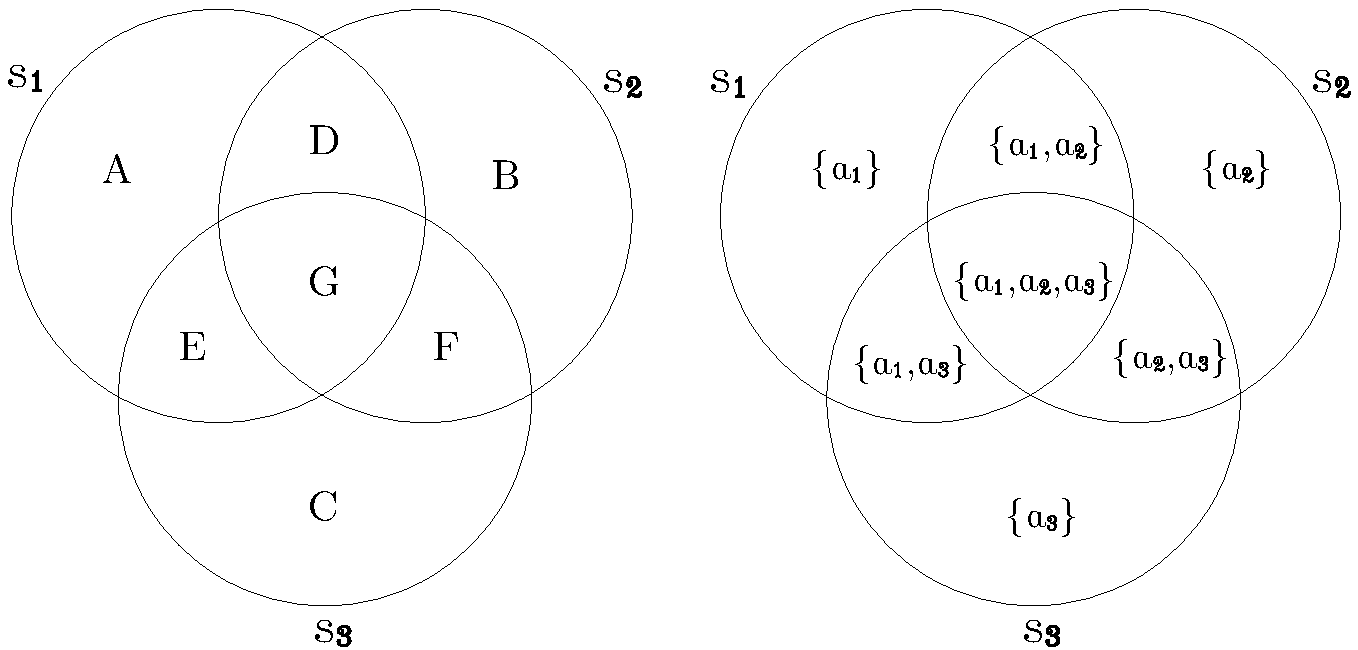
\includegraphics[scale=0.5]{fig-partitions-1.pdf}
    \caption{Partitions and Actions}
    \label{fig-partition-1}
\end{figure}

ELABORATE AND GIVE EXAMPLES(3)

\begin{algorithm}[H]
\SetAlgoLined
\SetKwInput{KwInput}{Input}
\SetKwInput{KwOutput}{Output}
\KwInput{$R = \{(s_1,a_1),...,(s_n,a_n)\}$}
\KwOutput{$P = \{(p_1,A_1),...,(p_m,A_m)\}$}
$P \leftarrow \{\}$\;
\For{each $T \subseteq R$}
{
   $S   \leftarrow \{s_k \se|\se (s_k,a_k) \in T\}$             \;
   $S'  \leftarrow \{s_l \se|\se (s_l,a_l) \in R\backslash T\}$ \;
   $A_i \leftarrow \{a_k \se|\se (s_k,a_k) \in T\}$             \; 
   $p_i \leftarrow \Big(\bigcap\limits_{s_k \in  S} s_k \Big)  
                   \Big\backslash 
                   \Big(\bigcup\limits_{s_l \in S'} s_l \Big)$   \;
   \If{$p_i \neq \varnothing$}
   {
      Add $(p_i, A_i)$ to $P$ \;
   }
}

\For{each $(p_x,A_x),(p_y,A_y) \subseteq P$}
{
   \If{$A_x = A_y$}
   {
      Remove $(p_x,A_x)$ and $(p_y,A_y)$ from $P$\;
      Add $(p_x \cup p_y, A_x)$ to $P$ \;
   }
}
\caption{Transforms a Rule Set to a Partition-Actions Set}
\end{algorithm}


\begin{definition2}[Compatibility of Two Partition-Actions Sets] Two partition-actions sets, 
$P=\{(p_i,A_i)\}$ and $P'=\{(p'_j,A'_j)\}$, are compatible if for all $c \in scope(P) \cup 
scope(P')$ there is a $(p_i, A_i)\in P$ and a $(p'_j,A'_j) \in P'$  such that $c\in p_i$,
$c\in p'_j$, and $A_i=A'_j$.
\end{definition2}

\begin{figure}
\begin{algorithm}[H]
\SetAlgoLined
\SetKwInput{KwInput}{Input}
\SetKwInput{KwOutput}{Output}
\KwInput{$P = \{(p_1,A_1),...,(p_n,A_n)\}, P' = \{(p'_1,A'_1),...,(p'_m,A'_m)\}$}
\KwOutput{True or False}
$s  \leftarrow scope(P)$\;
$s' \leftarrow scope(P')$\;
$P  \leftarrow \{(p_1\cap s', A_1),...,(p_n\cap s', A_n)\}$\;
$P' \leftarrow \{(p'_1\cap s, A'_1),...,(p'_n\cap s, A'_m)\}$\;
\eIf{$P = P'$}
{
   return true;
}
{
   return false;
}
\caption{$Compatible(P,P')$}
\end{algorithm}
\caption{Checks for Compatibility of Two Partition-Actions set}
\end{figure}


\begin{definition2}[Common Transition Set]
\end{definition2}



\begin{algorithm}[H]
\SetAlgoLined
\SetKwInput{KwInput}{Input}
\SetKwInput{KwOutput}{Output}
\KwInput{$\{R_1,...,R_p\}$}
\KwOutput{$R_0$}
$R_0 \leftarrow \{\}$\;
\For{each $R \in \{R_1,...,R_p\}$}
{
   $R_0 \leftarrow Merge(R_0,R)$\;
}
return $R_0$\;
\caption{Homogenization Algorithm}
\end{algorithm}

\begin{algorithm}[H]
\SetAlgoLined
\SetKwInput{KwInput}{Input}
\SetKwInput{KwOutput}{Output}
\KwInput{$R_x,R_y$}
\KwOutput{$R_z$}
Convert rule set $R_x$ to partition-actions set $P_x$\;
Convert rule set $R_y$ to partition-actions set $P_y$\;
\eIf{$P_x$ is compatible with $P_x$}
{
   $R_Z \leftarrow R_x \cup R_y$\;
}
{
   Match $P_x$ and $P_y$\; 
   \For{each $(p_i,A_i) \in P_x$ and each $(p_j,A_j) \subseteq P_y$}
   {
   }
}
return $R_Z$\;
\caption{Merging Two Rule Sets}
\end{algorithm}


\begin{algorithm}[H]
\SetAlgoLined
\SetKwInput{KwInput}{Input}
\SetKwInput{KwOutput}{Output}
\KwInput{$(p,A=(\alpha,\beta)),(p',A'=(\alpha',\beta'))$}
\KwOutput{(matching parameters)/no match}

\eIf{$\beta \neq \beta'$}
{
   return `no match'\;
}
{
   Solve $u_1\alpha+v_1=u_2\alpha'+v_2$\;
   //This linear diophantine equation is solved using Euclidean GCD algorithm\;
}
return $(u_1,v_1,u_2,v_2)$\;
\caption{Matching of Two Partition-Actions Pairs}
\end{algorithm}

% ================================================================================================================================================== %

\bibliographystyle{splncs03}
\bibliography{homonegenous-snp}

\end{document}





























